\documentclass[11pt,twoside,openany,x11names,svgnames]{memoir}
\usepackage[utf8]{inputenc}
\usepackage[latin1]{inputenc}
\usepackage[T1]{fontenc}
\usepackage[french]{babel}
\usepackage{graphicx}
\usepackage{array}
\usepackage{amsmath}
\usepackage{amssymb}
\usepackage{mathrsfs}
\usepackage{lmodern}
\usepackage{wallpaper}
\usepackage{tikz}
\usetikzlibrary{shapes,positioning}
\title{\textsl{\textbf{Auteurs:}}}
\author{CHAHOUD Marwane \\ ElGAMRANI Youssef \\ ELFAKIR Mehdi}
\date{29 Mai 2015}
\maketitle




%% Custom stock paper and page size
\setstocksize{303mm}{216mm}
\settrimmedsize{\stockheight}{\stockwidth}{*}

%% Adjust margins around typeblock
\setlrmarginsandblock{23mm}{18mm}{*}
\setulmarginsandblock{23mm}{23mm}{*}

%% Header and footer heights
\setheadfoot{\baselineskip}{10mm}
\setlength\headsep{7mm}

%% To apply and enforce layout
\checkandfixthelayout

%% Command to hold chapter illustration image
\newcommand\chapterillustration{}

%% Define a fancy chapter style
\makechapterstyle{FancyChap}{
%% Vertical Space before main text starts
\setlength\beforechapskip{0pt}
\setlength\midchapskip{0pt}
\setlength\afterchapskip{137mm}
%% Will print chapter number and title
%% in one go ourselves
\renewcommand*\printchaptername{}
\renewcommand*\printchapternum{}
%%% Re-define how the chapter title is printed
\def\printchaptertitle##1{
%% Background image at top of page
\ThisULCornerWallPaper{1}{\chapterillustration}
%% Draw a semi-transparent rectangle across the top
\tikz[overlay,remember picture]
  \fill[fill=LightSalmon1,opacity=.7]
  (current page.north west) rectangle 
  ([yshift=-3cm] current page.north east);
  %% Check if on an odd or even page
  \strictpagecheck\checkoddpage
  %% On odd pages, "logo" image at lower right
  %% corner; Chapter number printed near spine
  %% edge (near the left); chapter title printed
  %% near outer edge (near the right).
  \ifoddpage{
    \ThisLRCornerWallPaper{.35}{fern_mo_01}
    \begin{tikzpicture}[overlay,remember picture]
    \node[anchor=south west,
      xshift=20mm,yshift=-30mm,
      font=\sffamily\bfseries\huge] 
      at (current page.north west) 
      %{\chaptername\chapternamenum\thechapter};
    \node[fill=Sienna!80!black,text=white,
      font=\Huge\bfseries, 
      inner ysep=12pt, inner xsep=20pt,
      rounded rectangle,anchor=east, 
      xshift=-20mm,yshift=-30mm] 
      at (current page.north east) {##1};
    \end{tikzpicture}
  }
	%% On even pages, "logo" image at lower left
  %% corner; Chapter number printed near outer
  %% edge (near the right); chapter title printed
  %% near spine edge (near the left).
  \else {
    \ThisLLCornerWallPaper{.35}{fern_mo_01}
    \begin{tikzpicture}[overlay,remember picture]
    \node[anchor=south east,
      xshift=-20mm,yshift=-30mm,
      font=\sffamily\bfseries\huge] 
      at (current page.north east)
      {\chaptername\chapternamenum\thechapter};
    \node[fill=Sienna!80!black,text=white,
      font=\Huge\bfseries,
      inner sep=12pt, inner xsep=20pt,
      rounded rectangle,anchor=west,
      xshift=20mm,yshift=-30mm] 
      at ( current page.north west) {##1};
    \end{tikzpicture}
  }
  \fi
}
}


%% Define a fancy chapter style for unnumbered
%% chapters (e.g. the Table of Contents)
\makechapterstyle{FancyUnnumberedChap}{
%% Vertical Space before main text starts
\setlength\beforechapskip{0pt}
\setlength\midchapskip{0pt}
\setlength\afterchapskip{47mm}
%% Will print chapter number and title
%% in one go ourselves
\renewcommand*\printchaptername{}
\renewcommand*\printchapternum{}
%%% Re-define how the chapter title is printed
\def\printchaptertitle##1{
%% Draw a semi-transparent rectangle across the top
\tikz[overlay,remember picture]
  \fill[fill=LightSalmon1,opacity=.7]
  (current page.north west) rectangle 
  ([yshift=-3cm] current page.north east);
  %% Check if on an odd or even page
  \strictpagecheck\checkoddpage
  \ifoddpage{
    \begin{tikzpicture}[remember picture, overlay]
    \node[fill=Sienna!80!black,text=white,
      font=\Huge\bfseries, 
      inner ysep=12pt, inner xsep=20pt,
      rounded rectangle,anchor=east, 
      xshift=-20mm,yshift=-30mm] 
      at (current page.north east) {##1};
    \end{tikzpicture}
  }
  \else {
    \begin{tikzpicture}[remember picture, overlay]
    \node[fill=Sienna!80!black,text=white,
      font=\Huge\bfseries,
      inner sep=12pt, inner xsep=20pt,
      rounded rectangle,anchor=west,
      xshift=20mm,yshift=-30mm] 
      at ( current page.north west) {##1};
    \end{tikzpicture}
  }
  \fi
}
}


%% Set the uniform width of the colour box
%% displaying the page number in footer
%% to the width of "99"
\newlength\pagenumwidth
\settowidth{\pagenumwidth}{99}

%% Define style of page number colour box
\tikzset{pagefooter/.style={
anchor=base,font=\sffamily\bfseries\small,
text=white,fill=Sienna!80!black,text centered,
text depth=17mm,text width=\pagenumwidth}}

%% Concoct some colours of our own
\definecolor[named]{GreenTea}{HTML}{CAE8A2}
\definecolor[named]{MilkTea}{HTML}{C5A16F}

%% Sometimes I prefer not to upper-case my
%% running headers
\nouppercaseheads

%%%%%%%%%%
%%% Re-define running headers on non-chapter odd pages
%%%%%%%%%%
\makeoddhead{headings}
%% Left header is empty but I'm using it as a hook to paint the
%% background rectangles underneath everything else
{\begin{tikzpicture}[remember picture,overlay]
\fill[MilkTea!25!white] (current page.north east) 
	rectangle (current page.south west);
\fill[white, rounded corners] 
	([xshift=-10mm,yshift=-20mm]current page.north east) rectangle 	
	([xshift=15mm,yshift=17mm]current page.south west);
\end{tikzpicture}}%
%% Blank centre header
{}%
%% Display a decorate line and the right mark (chapter title)
%% at right end
{\begin{tikzpicture}[xshift=-.75\baselineskip,yshift=.25\baselineskip,remember picture, overlay,fill=GreenTea,draw=GreenTea]\fill circle(3pt);\draw[semithick](0,0) -- (current page.west |- 0,0);\end{tikzpicture}\sffamily\itshape\small\rightmark}

%%%%%%%%%%
%%% Re-define running footers on odd pages
%%% i.e. display the page number on the right
%%%%%%%%%%
\makeoddfoot{headings}{}{}{%
\tikz[baseline]\node[pagefooter]{\thepage};}
\makeoddfoot{plain}{}{}{\tikz[baseline]\node[pagefooter]{\thepage};}

%%%%%%%%%%
%%% Re-define running headers on non-chapter even pages
%%%%%%%%%%
\makeevenhead{headings}
%% Draw the background rectangles; then the left mark (section
%% title) and the decorate line
{{\begin{tikzpicture}[remember picture,overlay]
\fill[MilkTea!25!white] (current page.north east) rectangle (current page.south west);
\fill[white, rounded corners] ([xshift=-15mm,yshift=-20mm]current page.north east) rectangle ([xshift=10mm,yshift=17mm]current page.south west);
\end{tikzpicture}}%
\sffamily\itshape\small\leftmark\ 
\begin{tikzpicture}[xshift=.5\baselineskip,yshift=.25\baselineskip,remember picture, overlay,fill=GreenTea,draw=GreenTea]\fill (0,0) circle (3pt); \draw[semithick](0,0) -- (current page.east |- 0,0 );\end{tikzpicture}}{}{}
\makeevenfoot{headings}{\tikz[baseline]\node[pagefooter]{\thepage};}{}{}
\makeevenfoot{plain}{\tikz[baseline]\node[pagefooter]{\thepage};}
%% Empty centre and right headers on even pages
{}{}








\begin{document}

\newpage
\\
\\ \\ \\ \\ \\
\begin{figure}[h]
	\centering
		
\includegraphics[width=0.5\textwidth]{logo_ensa_uit.png}
	\label{}
\end{figure}
\begin{center}
\huge{\textbf{Université Ibn Tofail\\ \`Ecole Nationale Des Sciences Appliquées}}
\end{center}
\\
\newpage

\frontmatter

%%%%%%%%%%%%%%
%% Cover page
%%%%%%%%%%%%%%

%% No header nor footer on the cover
\thispagestyle{empty}

%% Cover illustration
%\ThisLLCornerWallPaper{1}{grapes-in-my-studio-little-too-much-dust}

%% Bar across the top
\tikz[remember picture,overlay]%
\node[fill=Sienna,text=white,font=\LARGE\bfseries,text=Cornsilk,%
minimum width=\paperwidth,minimum height=10em,anchor=north]%
at (current page.north){Travail d'Initiative Personnelle Encadré};

\vspace*{2\baselineskip}

%{\bfseries\itshape\color{LightGoldenrod!50!Gold}\fontsize{36pt}{46pt}\selectfont
%The Wonderful Calmness\par
%of Still Life Photos\par}

\vspace*{2\baselineskip}

%{\LARGE\color{LightGoldenrod}
%A small dummy example book by \scshape{Curutari}\par
%}

\tikz[remember picture,overlay]%
\node[fill=Sienna,font=\LARGE\bfseries,text=Cornsilk,%
minimum width=\paperwidth,minimum height=10em,anchor=south]%
 at (current page.south) {Sujet: Big Data};

\begin{center}
\LARGE\bfseries\color{SaddleBrown!30!black}

\end{center}

\cleartorecto

%% Invoke fancy unnumbered chapter style
%% for the table of contents
\chapterstyle{FancyUnnumberedChap}
%\tableofcontents*

%% Main matter starts here; resets page-numberings to arabic numeral 1
\mainmatter


{\bfseries\itshape\color{LightGoldenrod!25!Brown}\fontsize{40pt}{46pt}\selectfont
Remerciement \par
\par}
\begin{center}
\large{\textbf{Au terme de ce travail, nous saisissons cette occasion pour exprimer nos vifs remerciements à toute personne ayant contribué, de près ou de loin, à la réalisation de ce travail.\paragraph{}
En premier lieu, nous remercions nos parents; pour leur disponibilité, leur aide et leur soutien permanant.\paragraph{}
Nous tenons aussi à remercier chaleuresement tous ceux qui nous ont guidé et soutenu tout au long de ces trois mois et nos collègues, principalement \textit{Mr.Moulay Taïb BELGHITI} qui ne cessait jamais de nous donner ses conseils contructifs, ainsi nos vifs remerciement couvre l'ensemble du corps enseignant de l'\`Ecole nationnale Des Sciences Appliquées de Kénitra et sans oublier l'agent de sécurité \textit{Moustafa MAHHA}.\paragraph{}}}
\end{center}
\newpage
\tableofcontents





%%%%%%%%%%%%%%%%%%%%%%%%%%% MEHDI(& les AUTRES) EVITE COPIER/COLLER !! rak ma3roof :D %%%%%%%%%%%%%%%%%%%%%%%%%%%%%

     %%%%%%%%%%%%%%%%==> Synthétisiw dakchi !! f kola section wla subsection 1 tal 2 page maximum %%%%%%%%%%%%%%
						
					%%%%%%%%%%%%%%%%%%%%%%%%%%%%%%	Goood Luck !  %%%%%%%%%%%%%%%%%%%%%%%%%%%
\chapter{Big Data}
		\section{L'histoire du big data}
		\normalsize{ 1940-70 – Octets Il était une fois la Statistique : une question, (i.e. biologique),
associée à une hypothèse expérimentalement réfutable, une expérience planifiée avec $n=30$ individus observés sur p (moins de 10) variables, un modèle linéaire supposé vrai, un test, une décision, une réponse.

1970s – kO Les premiers outils informatiques se généralisant, l’analyse des données en France, (multivariate statistics ailleurs : Mardia et al. (1979) [5]) explore, prétendument sans modèle, des données plus volumineuses.

1980s – MO En Intelligence Artificielle, les systèmes experts expirent, supplantés par l’apprentissage (machine learning) des réseaux de neurones. La Statistique aborde des modèles non-paramétriques ou fonctionnels.

1990s – GO Premier changement de paradigme. Les données ne sont plus planifiées, elles sont préalablement acquises et basées dans des entrepôts pour les objectifs usuels (i.e. comptables) de l’entreprise. L’aide à la décision les valorise : From Data Mining to Knowledge Discovery (Fayyad etal., 1996)[2]. Les logiciels de fouille regroupent dans un même environnement des outils de gestions de données, des techniques exploratoires et de modélisation statistique). C’est l’avènement du marketing quantitatif et de la gestion de la relation client (GRC ou CRM).

2000s –TO Deuxième changement de paradigme. Le nombre p de variables explose (de l’ordre de 104 à 106), notamment avec les biotechnologies omiques où {$p\gg n$}. L’objectif de qualité de prévision l’emporte sur la
réalité du modèle devenu “boîte noire”. Face au fléau de la dimension, Apprentissage Machine et Statistique s’unissent en Apprentissage Statistique (statistical learning, Hastie et al. 2001-2009)[3] : sélectionner des modèles en équilibrant biais vs. variance ; minimiser conjointement erreurs d’approximation (biais) et erreur d’estimation (variance).

2010s – PO Troisième changement de paradigme. Dans les applications industrielles,
le e-commerce, la géo-localisation... c’est le nombre n d’individus qui explose, les bases de données débordent, se structurent en nuages (cloud), les moyens de calculs se groupent (cluster), mais la puissance brute ne suffit plus à la voracité (greed) des algorithmes.Un troisième terme d’erreur est à prendre en compte : celle d’optimisation, induite par la limitation du temps de calcul ou celle du volume / flux de données considéré. La décision devient adaptative ou séquentielle.}
		
				\subsection{Malédiction de la dimension}
				
				\normalsize On représente un ensemble des données par un vecteur $x$, tel que: \[x \in {I\!R^d},d \gg {10^6}\]
				
				
				\normalsize la malédiction de la dimension rend très difficile la détection ou la classification de ces données, car le volume est une fonction exponentielle. 
				
				Dans un espace de dimension 10, il faudrait $10^{20}$ points pour échantillonner un cube de largeur 1 avec des points dont la distance est $10^{-2}$.\\
		
		En dimension d il en faut $10^{2d}$, autrement dit un nombre inimaginable pour $d=10^{6}$.
		
		\section{Définition du Big Data}
		
		\normalsize Chaque jour, nous générons 2,5 trillions d’octets de données. A tel point que
	la majorités des données dans le monde ont été créées au cours des dernières années seulement. Ces données proviennent de partout : de capteurs utilisés pour collecter les informations climatiques, de messages sur les sites de médias sociaux, d'images numériques et de vidéos publiées en ligne, d'enregistrements transactionnels d'achats en ligne et de signaux GPS de téléphones mobiles, pour ne citer que quelques sources. Ces données sont appelées Big Data ou volumes massifs de données.
	on peut aussi definir le Big-data par l'ensemble de technologies, d’outils et de procédures qui permettent à une organisation de stocker, créer, manipuler, gérer et analyser très rapidement – voire en temps réel – ces grandes quantités de données et ces contenus hétérogènes, pour en extraire des informations pertinentes. 
		
		
		\section{Les 5V de la big data }
				\subsection{Volume}
				\normalsize Se réfère aux vastes quantités de données générées chaque seconde. Il suffit de penser de tous les e-mails, messages Twitter, des photos, des clips vidéo, des données de capteurs, etc. que nous produisons et nous partageons chaque seconde. Nous ne parlons pas téraoctets mais zettabytes ou Brontobytes. Sur Facebook seule nous envoyons 10 milliards de messages par jour, cliquez sur le «boutton commentaire» touche 4,5 milliards de fois et transférer $350$ millions nouvelles photos chaque jour. Si nous prenons toutes les données générées dans le monde depuis l'apparition d'internet et $2008$, le même quantité de données va bientôt être généré à chaque minute! Cela rend de plus en plus des ensembles de données trop grand pour stocker et analyser en utilisant la technologie de base de données traditionnelle. Grâce à la technologie grande de données, nous pouvons maintenant stocker et utiliser ces ensembles de données à l'aide de systèmes distribués, où des parties de les données sont stockées dans des emplacements différents et réunis par logiciel.
				\subsection{Velocity}
				\normalsize Se réfère à la vitesse à laquelle de nouvelles données est généré et la vitesse à laquelle les données se déplace autour. Il suffit de penser de messages de médias sociaux vont virale en quelques secondes, la vitesse à laquelle les transactions par carte de crédit sont vérifiées pour les activités frauduleuses, ou les millisecondes il faut des systèmes de négociation pour analyser les réseaux de médias sociaux pour capter les signaux qui déclenchent les décisions d'acheter ou de vendre des actions. Big technologie de données nous permet désormais d'analyser les données pendant qu'il est généré, sans jamais mettre en bases de données.
				\subsection{Variety}
				 \normalsize Dans le passé, nous nous sommes concentrés sur les données structurées qui convient parfaitement dans des tableaux ou des bases de données relationnelles, telles que les données financières (par exemple, les ventes par produit ou par région). En fait, la majorités des données du monde est maintenant non structuré, et ne peut donc être facilement mis en tables (penser à des photos, des séquences vidéo ou des mises à jour de médias sociaux). Grâce à la technologie grande de données, nous pouvons maintenant exploiter des types différentes de données (structurées et non structurées), y compris les messages, les conversations sur les médias sociaux, les photos, les données du capteur, vidéo ou des enregistrements vocaux et de les réunir avec des données plus traditionnelles, structurées.
				\subsection{Veracity}
				 \normalsize Se réfère au désordre ou la fiabilité des données. Avec de nombreuses formes de données grande, la qualité et la précision sont moins contrôlables (il suffit de penser messages aux Twitter avec les balises de hachage, les abréviations, les fautes de frappe et le discours familier ainsi que la fiabilité et l'exactitude du contenu), mais les grandes données et la technologie d'analyse maintenant nous permet de travailler avec ce type de données. Les volumes constituent souvent le manque de qualité ou l'exactitude.
				\subsection{Valeur}
				\normalsize Puis il y a un autre V à prendre en compte quand on regarde Big Data: Valeur! Il est bien beau d'avoir accès à des données importantes mais si nous ne pouvons le transformer en valeur, il est inutile. Ainsi, vous pouvez argumenter en toute sécurité que la «valeur» est le V le plus important de Big Data. Il est important que les entreprises font une analyse de rentabilisation pour toute tentative visant à collecter et exploiter des données importantes. Il est si facile de tomber dans le piège de buzz et de se lancer sur les initiatives grands de données sans une compréhension claire des coûts et des avantages.

				
		\section{Définition d'une base de donnée.}
\subsection{Définition}
\normalsize Une base de donnée (BD) est un ensemble bien structurée et organisé permettant le stockage des données
afin de faciliter l’exploitation (ajout, suppression, mise à jours ....). 
La phrase base de donnée est composée de deux mot base et donnée, base signifie l'endroit ou l'espace dans lequel on veut stocker et gérer nos données, et donnée signifie les données ciblés .Donc on a un endroit qui contient nos données 
\includegraphics{bd.gif} 
\normalsize On peut stocker nos données sont utilisé une bd alors pourquoi utilisons-nous cette dernière ?
pour répondre à cette question on doit ouvrir la parhentése sur l'utilité des bases de données , à quel point ces derniers nous servent .\paragraph{}                                                                    
\subsection{L'utilité d'une base de données}

\normalsize Une base de données permet de mettre des données à la disposition d'utilisateurs 
pour une consultation, une saisie ou bien une mise à jour, tout en s'assurant des droits accordés 
à ces derniers. Cela est d'autant plus utile que les données informatiques sont de plus 
en plus nombreuses. 
Une base de données peut être locale, c'est-à-dire utilisable sur une machine 
par un utilisateur, ou bien répartie, c'est-à-dire que les informations sont stockées 
sur des machines distantes et accessibles par réseau. 
L'avantage majeur de l'utilisation de bases de données est la possibilité de pouvoir 
être accédées par plusieurs utilisateurs simultanément. 

				\subsection{SGBD ?}
				\normalsize Jusqu'à maintenant on a bien sentis le rôle des BD et à quoi servent-t-elles ,mais on sait pas comment gérer les données et controler les utilisateurs (peut importe peut accéder à nos données ?..).
				Afin de pouvoir contrôler les données ainsi que les utilisateurs, le besoin d'un 
Système de gestion s'est vite fait ressentir. 
La gestion de la base de données se fait grâce à un système appelé système de gestion de bases de données SGBD ou en anglais DBMS (Database management system).
SGBD ce sont des applications logicielles permettant de gérer les
bases de données, c'est-à-dire :

-Permettre l'accès aux données de façon simple.\paragraph{}
-Autoriser un accès aux informations à de multiples utilisateurs.\paragraph{}
-Manipuler les données présentes dans la base de données (insertion, suppression, modification).\paragraph{}
\normalsize Ils existent plusieurs programmes qui font ce travaille : Oracle, Mysql, Postgresql, Microsoft Access...
				
				\subsection{NoSQL ?}
				
				\normalsize Après avoir définir qu'est ce que c'est une BD et expliquer le SGDB revenons à notre sujet le BIG DATA .
			Qui sont les SGBD utilisé pour BIG DATA ?
								il existe plusieurs SGBD et parmi ces dernières il y a le NoSQL .
NoSQL signifie “Not Only SQL". Ce terme désigne l’ensemble des bases de données qui s’opposent à la notion relationnelle des SGBDR. La définition, “pas seulement SQL”, apporte un début de réponse à la question “Est-ce que le NoSQL va tuer les bases relationnelles?”. En effet, NoSQL ne vient pas remplacer les BD relationnelles mais proposer une alternative ou compléter les fonctionnalités des SGBDR pour donner des solutions plus intéressantes dans certains contextes.\paragraph{}
	\textbf{Pourquoi choisissons-nous le NoSQL ?}\paragraph{}
	\\
				\textbf{Avantages}

\normalsize L’intérêt des systèmes de stockage NoSQL réside surtout dans les choix d’architecture logicielle qui ont été pris lors de leurs conceptions. Parmi les raisons principales qui ont mené à la création de ces systèmes, on retrouve surtout deux points principaux :
La possibilité d’utiliser autre chose qu’un schéma fixe sous forme de tableaux dont toutes les propriétés sont fixées à l’avance ;
La possibilité d’avoir un système facilement distribué sur plusieurs serveurs et avec lequel un besoin supplémentaire en stockage ou en montée en charge se traduit simplement par l’ajout de nouveaux serveurs.
	
				
			\subsection{Data-mining ?}
			\normalsize Le Data-mining est un domaine interdisciplinaire qui utilise des techniques d’apprentissage automatique, de la reconnaissance des formes, des statistiques, des bases de données et de la visualisation pour l'extraction d'informations à partir de bases de données volumineuses .
				\subsection{Datawarehouse ?} 
				\normalsize Un Datawarehouse est une serveur informatique permet de collecter, ordonner, journaliser et stocker les informations , dans laquelle les données sont bien organisées pour faciliter l'accès par les utilisateurs . 
					
				\subsection{Problématique du Big Data}
				
Les données volumineuses sont au coeur des problématiques émergentes de recherche, en faisant notamment appel à des structures de données sophistiquées : graphes, fonctions, variétés. Chaque problème est porteur de sa propre originalité ; ce projet se limite aux articulations: Statistique, Apprentissage supervise et non supervise.

En plus il faut savoir que le big data n’est pas un problème technique, le problème c'est que La minorité des entreprises qui peut targuer (avoir des avantages) d’une maturité élevée de son exploitation des DATA parce que le volume des données numériques augmente d’une façon exponentielle(malédiction de dimension).Et malgré ces problèmes Il existe des logiciels utilisé par les grands sociétés tel que Facebook ,Google,E-bay,Amazon,... capables de traiter les données (Hadoop ,Mapreduce…).
 Le défi est technologique et scientifique.\\
\textbf{ Comment stocker, archiver ces données, les rendre lisibles et exploitables ?}

 \newpage
\begin{center}


\tikz[remember picture,overlay]%
\node[fill=Sienna,text=white,font=\LARGE\bfseries,text=Cornsilk,%
minimum width=\paperwidth,minimum height=5em,anchor=middle]%
at (current page.middle){
\fbox{
\begin{minipage}{1\textwidth}
\textsl{« Demandez à n’importe quel chief data officer de définir Big Data et il va se mettre à regarder ses chaussures. En réalité, il y a de forte chance pour que vous obteniez autant de définitions différentes que le nombre de personnes auxquelles vous poserez la question »} \par \\

 -MIT Review 7
\end{minipage}
} };
\end{center}



\newpage
\chapter{Cycle de vie des données}
     
		  
			\begin{figure}[h]
				\centering
					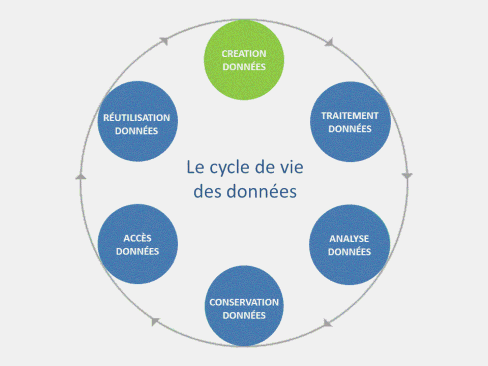
\includegraphics[width=0.80\textwidth]{o_fbc17caea503ddea-0.png}
				\caption{cycle de vie de données}
				\label{fig:o_fbc17caea503ddea-0}
			\end{figure}
			
		

Les données se multiplient à un rythme incroyable et parallèlement, notre dépendance à l’égard des archives ne fait que s’accentuer. Plus de 30 milliards d’e-mails sont échangés par jour dans le monde, et ce n’est qu’un exemple de la multitude de supports auxquels les entreprises doivent accéder à la demande. 
		 \section{Collection ou création des données :}
			Construire une base de données nécessite de collecter une multitude d’informations provenant des sources différentes et utilisateurs différents.
				\section{Traitement}
		Cette \'etape consiste à traiter les données collect\'es dans l'étape pr\'ecedente, ce qui est difficile à faire, vue la taille des données collect\'es. cette étape présente un problème intéressant au Big-data.
				
				
		\section{Analyse}
		
		\`A cette étape, les données sont prêtes à être analysé. Les applications du Big data varient selon l’utilisation de chaque organisation ou entreprise. On peut distinguer trois utilisations majeures :
		
			\begin{itemize}
	\item \textbf{Détecter et optimiser :} \\
				La production en masse et le croisement des données en temps réel permettent une compréhension et une vision claire sur l’environnement. Par exemple la prise de décision.
	\item \textbf{Tracer et cibler :} \\
				La granularité des données analysées permet le suivi à un niveau très fin, par exemple : avoir des informations sur un individu dans une population.
	\item \textbf{Prévoir et prédire :} \\
	La variété des données disponibles sur un phénomène ou une population permettent de construire des modèles prédictifs (analyse prédictive, voir aussi théorie des jeux). Ce fonctionnement s’inscrit dans les pas du Datawarehouse(entrepôt de données).
	 
		
		\section{Conservation des donn\'ees:}
		 Cette étape est aussi interressante , son but est de conserver les donn\'ees traiter et analyser aux étapes précedente .
		 
		
		
		\section{Acc\'ees:}
		 \`A fin de faire passer les données aux utilisateurs , il faut trouver des liaisons qui permettent de lies les bases de donn\'ees et l'utilisateur, par exemple : établir un serveur, iCloud, Dropbox....
		
\chapter{Domaine d'utilisation}
Le Big Data touche tous les domaines allant de l’industrie à la santé, en passant par la sécurité.
	\section{Médical}
			
			\normalsize Applications de l’analyse des volumes massifs de données dans le domaine de la santé sont aussi nombreuses que variées, dans la recherche comme dans la pratique. \\
Citons par exemple les systèmes de surveillance des patients à distance utilisés pour les maladies chroniques, qui peuvent permettre de limiter les rendez-vous chez le médecin, les visites dans les services d’urgence et les jours d’hospitalisation, de mieux cibler les soins et de prévenir certaines complications médicales à long terme.\\
L’analyse de grands ensembles de données contenant les caractéristiques des patients, les effets des traitements et leurs coûts peut contribuer à repérer les traitements les plus efficaces d’un point de vue clinique et sur le plan financier.  De plus, l’analyse des tableaux épidémiologiques à l’échelle mondiale en vue de dégager des tendances à un stade précoce est d’une importance critique, non seulement pour gérer les crises sanitaires, mais aussi pour permettre aux secteurs pharmaceutique et médical de modéliser la demande future pour leurs produits et, sur cette base, de prendre des décisions sur les investissements à faire en matière de recherche et développement.\\

		\section{Prédiction: Analyse prédictive}
		
		\normalsizeLes Techniques d’analyses avancées actuellement disponibles parmi lesquelles l’analyse prédictive, le text-mining, l’analyse sémantique ou encore le machine-learning sont indispensables pour permettre aux organisations de générer un véritable avantage compétitif grâce aux données analysées avec des niveaux de sophistication, de vitesse et précision impensables jusqu’à aujourd’hui. Même si une majorité d’organisations (plus de 75pour cent) s’appuie sur le data-mining pour exploiter les Big Data, un nombre toujours croissant (67pour cent) indique utiliser la modélisation prédictive. Le manque de compétences analytiques avancées est un frein majeur à l’exploitation plus approfondie des Big Data.\\
Les applications prédictives avancées reposent sur l’évaluation des risques et de la sensibilité, ce qui permet aux décideurs d’identifier les variables les plus importantes dans la prise de décision. Si, par  exemple, une variable se révèle critique dans la prise de décision, il est alors possible d’en vérifier  l’éxactitude et la globalité.\\
Exemples d’applications prédictives/prévisionnelles :


\begin{enumerate}
	\item Applications de test clinique qui modélisent l’effet de différents médicaments en fonction de tests cliniques afin que l’entreprise puisse comprendre l’efficacité de certains traitements et éviter les conséquences catastrophiques de l’utilisation de certaines associations médicamenteuses. 



	\item Applications de détermination de l’attrition des clients qui prévoient la probabilité d’attrition des clients en fonction de critères, tels que les activités d’utilisation, les demandes de support, les modèles de paiement et l’influence sociale des amis.
	
	\newpage


\tikz[remember picture,overlay]%
\node[fill=Sienna,text=white,font=\LARGE\series,text=Cornsilk,%
minimum width=\paperwidth,minimum height=5em,anchor=middle]%
at (current page.middle){
\fbox{
\begin{minipage}{1\textwidth}
\textsl{\underline{•	Prédiction en matière de crimes:} \\
«\textbf{Le logiciel \textbf{PredPol} ‘Predictive policing’} fonctionne sur un algorithme dessiné par un mathématicien, un anthropologue et un criminologue. En agrégeant des données diverses : démographie d’un quartier, historique des infractions, ... Les autorités policières peuvent distinguer les zones où les infractions les plus probables.
»} \par \\

\end{minipage}
} };
\end{center}

\newpage



	\item Applications de mesure des performances des employés qui prévoient les performances potentielles d’un employé en fonction de critères, tels que la formation, la classe socio-économique, l’historique des emplois précédents, l’état civil et des réponses psycho-comportementales.
	
\end{enumerate}
		\section{Finance,gestion,..}
						
						\normalsize L’évolution des connexions à haut débit dans le monde au cours de la dernière décennie a permis un changement radical des usages des consommateurs.  Cela donne lieu à des échanges massifs de données, si bien que, selon la définition d’IBM, le volume de ces données ne peut plus être traité avec les outils traditionnels. 
Toutes les informations stockées et collectées grâce au web s’inscrivent dans le cadre du Big Data : vos analytiques (analyses d’audience internet), vos bases de données clients, l’historique d’achat de vos clients, les différents parcours de navigation sur votre site, les données démographiques de vos visiteurs et les interactions de vos clients et prospects sur les réseaux sociaux sont autant de données qu’il est possible d’exploiter.
Ces données sont utilisés pour identifier les besoins des clients .

\section{Environnement : pic d’ozone}

L’objectif est de prévoir pour le lendemain les risques de dépassement de seuils de concentration d’ozone dans les agglomérations à partir de données observées : concentrations en $0_{3}, NO_{3}, NO_{2}$... du jour, et d’autres prédites par Météo-Monde : température, vent... \\ Encore une fois, le modèle apprend sur les dépassements observés afin de prévoir ceux à venir.

\section{Exemples industriels}


Depuis de très nombreuses années, l’industrie agroalimentaire est confrontée à des problèmes de grande dimension pour l’analyse de données de spectrométrie comme par exemple dans le proche infra-rouge (NIR).

\begin{figure}[h]
	\centering
		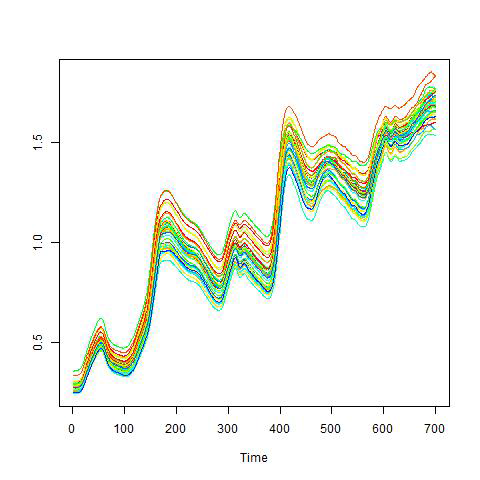
\includegraphics[width=0.80\textwidth]{imageee.png}
	\caption{ Spectres proche infrarouge (NIR)}
	\label{fig:imageee}
\end{figure}


				
				
\chapter{Loi de Moore "Moore's Law"}
		\section{Définition}
		Une loi relative à la croissance de la performance des ordinateurs (en générale: des microprocesseurs,microprocesseurs graphique). \\
		\'Enoncé depuis 50ans, Gorden Moore publie au sein du magazine Electronics un article portant sur ses observations dans le taux de croissance exponentiel des circuits intégrés. Constatant depuis 1959, un doublement régulier chaque 2ans, de nombre de transistors utilisé dans chaque composant éléctronique. Cela est d\^u à la miniaturisation des transistors. \\
		\textbf{\textsl{La formulation originelle:}}
	
 \fbox{
\begin{minipage}{1\textwidth}
{\textsl{"The complexity for minimum component costs has increased at a rate of roughly a factor of two per year ... Certainly over the short term this rate can be expected to continue, if not to increase. Over the longer term, the rate of increase is a bit more uncertain, although there is no reason to believe it will not remain nearly constant for at least 10 years. That means by 1975, the number of components per integrated circuit for minimum cost will be 65,000. I believe that such a large circuit can be built on a single wafer."}} 
\end{minipage}
}
\\
 \\
\newpage
\begin{figure}
	\centering
		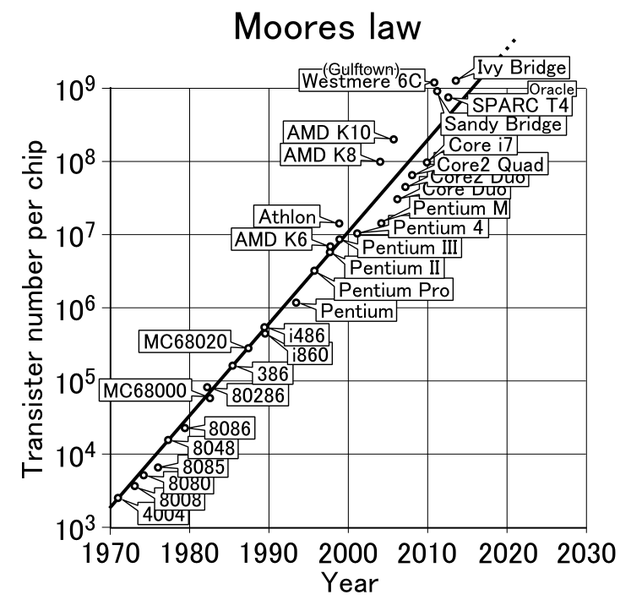
\includegraphics[width=0.5\textwidth]{642px-Moores_law_1970-2011.png}
	\label{fig:642px-Moores_law_1970-2011}
\end{figure}


 \\
Comme l'indique la figure à coté, le nombre de transistor double dans chaque processeur, ainsi que l'horloge. \\
Les algorithmes qu'on avait d\'eja vu et la multitude des données massive (à l'ordre de {$10^{21}$} zetaoctet) nécessite une machine
 doté d'une performance accrue pour le traitement de ces données. Aujourd'hui, un ordinateur qui
supportera cet algorithme est en cour de développement, gr\^ace à la loi de Moore, on pourrait avoir une idée
sur les ordinateurs/serveurs des génération qui suit, qui pourrant supporter le traitement en temp réel des données massives.

\newpage


\tikz[remember picture,overlay]%
\node[fill=Sienna,text=white,font=\LARGE\bfseries,text=Cornsilk,%
minimum width=\paperwidth,minimum height=5em,anchor=middle]%
at (current page.middle){
\fbox{
\begin{minipage}{1\textwidth}
\textsl{« Hadoop est composé d’une architecture de calculs parallèles et distribués nommée MapReduce. Modèle de programmation permet la manipulation des données en grand quantité distribuées sur le
cluster de noeuds de serveurs qui
composent l’architecture de la solution
Big Data déployée
»} \par \\

\end{minipage}
} };
\end{center}

\newpage
		
		
\chapter{Mahématique du Big Data}      
		\section{Algorithme supervisé}
		Dans ce chapitre nous allons nous intéresser essentiellement à l’apprentissage supervisé, pour lequel on dispose d’un ensemble d’apprentissage constitué de données d’observations de type entrée-sortie  $\[D_1^n = ({X_1};{Y_1});...;({X_n};{Y_n})\]$ ou ${X_{i} \in {I\!R}^{p}}$
		
		L’objectif est de construire, à partir de cet échantillon d’apprentissage, un
modèle, qui va nous permettre de prévoir la sortie $y$ associée à une nouvelle entrée (ou prédicteur) $x$.
La sortie $y$ peut être quantitative (prix d’un stock, courbe de consommation électrique, carte de pollution ..) ou qualitative (sur- venue d’un cancer, reconnaissance de chiffres...)

\textbf{sorties quantitatives} $Y\subset R^{p} \rightarrow r\acute{e}gression$


		\textbf{sorties qualitatives} $Y fini \rightarrow discrimination, classement$ \\
		Dans la suite, nous allons nous intéresser aux principes de fonctionnement de l'apprentissage supervisé. \\
		On distingue deux types de tâches réalisable à savoir:
		\begin{enumerate}
		\item {La classification}
		\item{La régression}
	
		\end{enumerate}
		\subsection{Classification}
		\textbf{La classification} est utilisé lorsque le label à prédire est \textbf{discret} et nous parlons de \textbf{régression} lorsque le label à prédire est \textbf{continu}.\\
		
		Concernant ce type de traitement nous allons étudier deux types d'algorithme pour illustrer le fonctionnement de la \textbf{classification}, qui sont: \\
		\begin{enumerate}
		\item {L'arbre de décision}
		\item{Support Vecteur Machine (SVM)}
		\end{enumerate} \\
		Des exemples d'application seront présent pour la bonne compréhension de cete partie. \\
		En va commencer par des notions en statistiques et illusterons le fonctionnement de ces algorithmes en utilisant le jeu de données Iris. \\ 
		\\
		{\large{\textbf{Jeu de données Iris:}}}
		\\
		Il s'agit d'un historique recensant les dimensions \textsl{(longueur des sépales, largeur des sépales, longueur des pétales et largeur des pétales)} de $150$ iris et l'espèce associée à chaque iris: \\
		
		\begin{figure}[h]
			\centering
				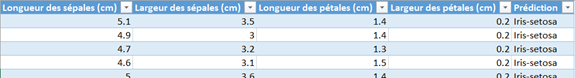
\includegraphics[width=0.75\textwidth]{img1_iris.png}
			\label{}
		\end{figure}
		
		
		%%%%%%%%%%%%%%%% JEU D'IRIS A FAIRE %%%%%%%%%%%%%%%%%%%
		
		
		\section*{\large{\textbf{\underline{Vocabulaire et notations en statistique:}}}} 
		\\
		
		\begin{enumerate}
		\item {{\large{\textbf{\underline{Variable aléatoire:}}}}} \\
		Dans le jargon mathématique, on apelle $X$ variable aléatoire qui change en fonction de ce qu'on appelle une réalisation $w$. \\
		
		%%%%%%%%%%%%%% TABLEAU illustratif de la variable aléatoire %%%%%%%%%%%
		
		\begin{figure}[h]
			\centering
				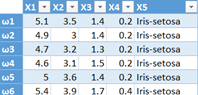
\includegraphics[width=0.35\textwidth]{img2_iris.png}
			\label{}
		\end{figure}
		Pour décrire la variable aléatoire $X$, on a : \\
		{\textbf{L'espérance:}} représente la moyenne selon les réalisations. \\
		
		\hspace{3cm} \textbf{\[E(X) = {\mu _X} = \frac{1}{{nombrede\omega }}\sum\limits_\omega  {X(\omega )} \]} \\
		
		{\textbf{L'écart-type:}} représente la dispersion des données: \\
		\hspace{3cm} \[{\sigma _X} = \sqrt{E(X^{2}) - (E(X)^{2})\]}
		
		\item{{\large{\textbf{\underline{Corrélation:}}}}} \\
		La corrélation est une mesure de la dépendance entre 2 variables aléatoires. Dans notre exemple, on remarque que la longueur des pétales est grande alors la largeur des pétales est grande. On dit qu'il y a une \textbf{corrélation positive} (c'est à dire il y a relation) entre la longueur et la largeur des pétales. Par contre, il n'y a pas de corrélation entre la longueur des sépales et la largeur des sépales, on dit alors que ce sont deux \textbf{deux variables indépendantes.} \\
		\begin{figure}[h]
			\centering
				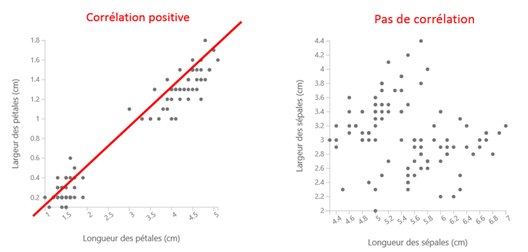
\includegraphics[width=0.6\textwidth]{img3_iris.png}
			\label{}
		\end{figure} \\
		Il est important de comprendre que la corrélation n'est qu'une mesure de la dépendance entre $2$ variables du même système etudié; cela n'implique pas nécessairement qu'il existe une causalité entre ces $2$ variables. \\
		
		
		\item{{\large{\textbf{\underline{Indicateurs de corrélation:}}}}} \\
		Pour mesurer la corrélation entre deux variables aléatoires $X et Y$, on retrouve: \\
		{\textbf{Le coefficient de corrélation linéaire de $Bravais-Pearson$:}} \\
		\hspace{3cm}{ \[corr(X,Y) = \frac{{\operatorname{cov} (X,Y)}}{{{\sigma _X}{\sigma _Y}}} = \frac{{\frac{1}{n}\sum\limits_{i = 1}^n {({x_i} - \bar x)({y_i} - \bar y)} }}{{{\sigma _X}{\sigma _Y}}}\] }
		\\
		tel que $\overline{x}$ et $\overline{y}$ sont les moyennes des séries $X$ et$Y$.  
		
		\end{enumerate} \\
		{{\large{\textbf{\underline{Application de l'algorithme:arbres de décision}}}}} \\
		Les algorithmes à base d'arbres de décision sont très populaires. Ils établissent des règles qui permettent de déterminer le label à prédire en fonction des caractéristiques. Appliquer ceci sur nos données donnerait un résultat de la forme: \\
		\hspace{3cm} \textsl{"Si la largeur des pétales est inférieur à 3,5, alors l'Iris est de type Iris-setosa, sinon l'iris est de type Iris-virginica"} \\
		
		Les arbres de décision ont l'avantage d'être aisément interprétables par un humain et trés rapidement applicables par une machine.\\
		{{\large{\textbf{\underline{Application à la main sur le jeu de données Iris:}}}}} \\
		On visualise les données de la manière suivante: \\
		
		
\begin{figure}[h]
			\centering
				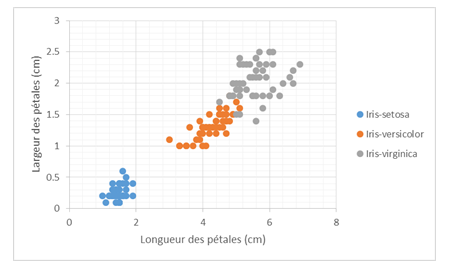
\includegraphics[width=0.5\textwidth]{img4_iris.png}
			\label{}
		\end{figure} \\
		
		Posons la règle suivante:\\
		\textsl{"Si la longueur des pétales est inférieure à $2$, alors l'iris est de type Iris-setosa"} \\
				
				\begin{figure}[h]
			\centering
				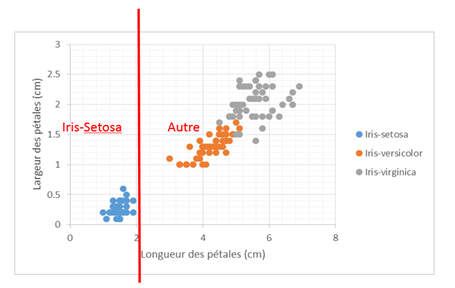
\includegraphics[width=0.5\textwidth]{img5_iris.png}
			\label{}
		\end{figure} \\
				Ensuite, il ne reste que l'attribut largeur des pétales à traiter. \\
				la régle est la suivante: \\
				\textsl{"Si la largeur des pétales est supérieure à $1.7$, alors l'iris est de type Iris-virginica, sinon il est de type Iris-versicolor"} \\
				
				\begin{figure}[h]
			\centering
				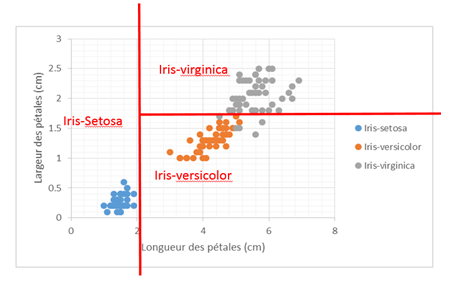
\includegraphics[width=0.55\textwidth]{img6_iris.png}
			\label{}
		\end{figure} \\
		\newpage
		L'arbre peut donc être visualisé sous la forme suivante: \\
		\begin{figure}[h]
			\centering
				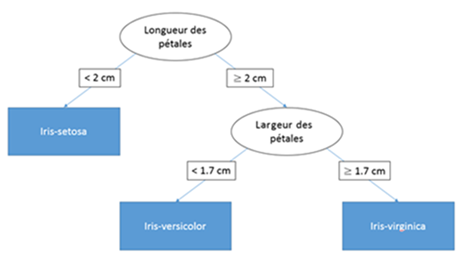
\includegraphics[width=0.5\textwidth]{img7_iris.png}
			\label{}
		\end{figure} \\
		
		{{\large{\textbf{\underline{Algorithme général:}}}}} \\
		
		L'algorithme se déroule de la maniére suivante: \\
		\begin{enumerate}
		\item Calculer la quantité d'information de chaque attribut, c'est à dire la corrélation de chaque attribut.
		\item Pour l'attribut qui apporte le plus d'information, choisir la meilleure règle \textsl{"Si A alors B"}: \\
		\hspace{2cm} \textsl{Déterminer A} \\
		\hspace{3cm} -Pour un attribut à valeurs discrètes, les valeurs de A pour chaque règle sont les valeurs prises par l'attribut. \\
		\hspace{3cm} - Pour un attribut à valeurs continues, A est le seuil qui classifie "au mieux" tous les éléments. En particulier, si tous les attributs sont continus, on obtient un arbre binaire. \\
		\hspace{2cm} \textsl{Déterminer B} \\
		\hspace{3cm} -Si la classe à prédire est la même pour toutes les réalisations lorsqu'on applique la rêgle "Si A", alors B est la classe à prédire. \\
		\hspace{3cm} -Sinon, B est une nouvelle règle déterminée en réappliquant cet algorithme sur les éléments restants.\\
		\end{enumerate}
		
		{{\large{\textbf{\underline{Deuxième algorithme:SVM}}}}} \\
		Les SVM s'appuient sur la notion de distance entre les données. Ces algorithmes sont très performants mais nécessitent beaucoup de temp de calcul.\\
		L'algorithme consiste à trouver la courbe qui \textbf{sépare au mieux} les données, c'est-à-dire, de telle sorte que tous les éléments au-dessous de cette courbe appartiennent à la classe1, tous les autres à la classe2.\\
		Toutefois, une infinité de courbes séparent les données. Il s'agit de trouver la meilleure. Pour cela, on utilise le \textbf{critère de marge maximale.}\\
		{{\large{\textbf{\underline{SVM linéaire-cas séparable:}}}}} \\
		Reprenons notre jeu de données iris. On recherche la meilleur droite qui sépare le mieux les Iris-setosa et les Iris-versicolor: \\
		%%%% Image %%%
\begin{figure}[htbp]
	\centering
		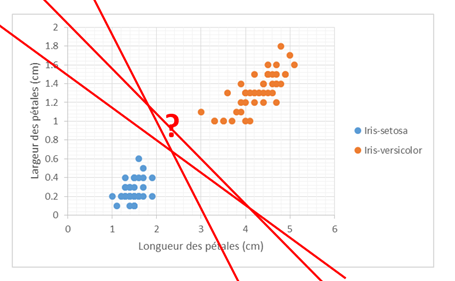
\includegraphics[width=0.55\textwidth]{img8_iris.png}
	\label{}
\end{figure} \\
Pour cela, on définit la \textbf{marge} comme la plus petite distance entre les points de chaque classe et le séparateur. Il est alors possible de choisir le meilleur séparateur comme étant celui maximisant la marge: \\

		\begin{figure}[htbp]
	\centering
		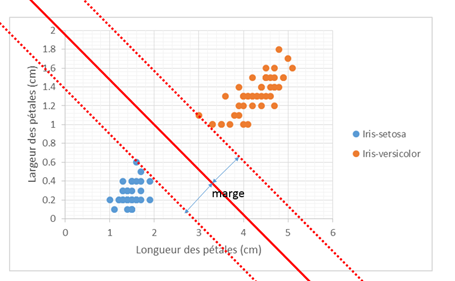
\includegraphics[width=0.55\textwidth]{img9_iris.png}
	\label{}
\end{figure} \\
Maximiser la marge permet d'obtenir un meilleur classifieur dans la mesure il faut rester conscient que les données d'apprentissage ne sont pas exhaustives.
		
		
		
		
		
		
				\subsection{Regressement}
				
							
				
			\textbf{Type de regression linéaire:}
			
			
			\begin{figure}[h]
				\centering
					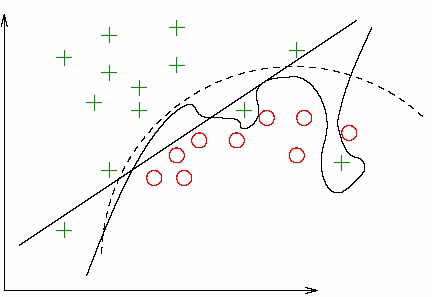
\includegraphics[width=0.82\textwidth]{Sans titre.png}
				\caption{Droite de regression lin\'eaire }
				\label{}
			\end{figure}
			
			     
					 
					 \begin{itemize}
		 \item\textbf{ Apprentissage supervisé avec des équations : }
	Pour évaluer la performance d’un classifieur f, on définit d’abord une fonction de coût $L$ qui va donner une mesure de l’erreur entre la prédiction $f(x)$ et la valeur réelle $y$. 
	En général, la fonction de coût est choisie comme le carré de l’écart au résultat à prédire, c’est l’approximation des moindres carrés :\\
						
						
						\hspace{3cm}\textbf{$L_{f}(x,y)=\left\|f(x)-y\right\|_{2}^{2}$} \\
						
						
						
	Ensuite, on définit une fonction erreur $R$ qui mesure la somme des écarts entre la valeur réelle $y$ et la prédiction $f(x)$.\\
					
					\hspace{3cm}\textbf{$ \[R(f) = \sum\limits_{i = 1}^n {{L_f}({x_i},{y_i}) = \sum\limits_{i = 1}^n {[f({x_i})} }  - {y_i}]^{2}\]$} \\
					
					
					où $n$ est le nombre d’éléments dans l’historique.
					
Alors, effectuer une régression consiste à trouver la fonction $f$ qui minimise l’erreur :\\
					
					    \hspace{3cm}\textbf{$\[f = \arg \min \sum\limits_{i = 1}^n {[f({x_i}) - {y_i}]} \]^{2}$} \\
							
						
							 \item\textbf{ Régression linéaire:}
					
					\begin{enumerate}
					
						
	
					 \item\textbf{ Régression simple - x est un scalaire :}
			
		La régression linéaire est une méthode d’apprentissage supervisé permettant d’estimer f en supposant que f a une forme linéaire :\\
					             
											
											\hspace{3cm}\textbf{$f(x)=ax+b$}
											
					
		Déterminer f consiste alors à trouver a et b en minimisant la fonction $R$ \\ 
					
		
			\hspace{3cm}\textbf{$\[(A,B) = \arg \min \sum\limits_{i = 0}^n {[(A \times {x_i} + B) - {y_i}]} \]^{2}$} \\
			
			
			
		 il est possible de résoudre cette équation à l’aide de la méthode du gradient.
					
									
		 \item\textbf{Régression multiple - x est un vecteur:}
	
		 
		dans ce cas  \hspace{3cm}\textbf{$f(x)=AX+B$}
		
				
	avec A un vecteur et B est un scalaire .
				
		La formule d’optimisation devient : \\
					
	\hspace{3cm}\textbf{$\[(A,B) = \arg \min \sum\limits_{i = 0}^n {[(A \times {x_i} + B) - {y_i}]} \]^{2}$} \\
	
					
	Ainsi, avec les notations vectorielles, on constate qu’il est facile de généraliser la plupart des méthodes appliquées à des scalaires. Toutefois, le temps de calcul est plus important car il y a plus de coefficients à évaluer (p+1 coefficients au lieu de 2).
			
	 \item\textbf{Régression multiple, notation matricielle :}
				
	Dans la littérature, on trouve souvent ces équations posées sous forme matricielle afin d’avoir une écriture condensée.

Posons $X$ la matrice constituée des $n$ vecteurs $x$, $Y$ la matrice constituée des $n$ vecteurs $y$. Alors A devient une matrice et on peut écrire :

                                \hspace{3cm}\textbf{$(A,B)=argmin\left\|AX-Y\right\|_{2}^{2}$}
		
					\end{enumerate}
					\end{enumerate}
		
         \end{enumerate}					
				
				
		\section{Algorithme non supervisé}
			\textbf{l'apprentissage non-supervisé , de quoi s'agit-il ?}\paragraph{}
		On parle d’apprentissage non-supervisé lorsque les données sur lesquelles on travaille ne sont pas labélisées, c’est-à-dire qu’il n’y a pas d’indication concernant l’attribut à prédire.\paragraph{}
		  Ils se servent de la distribution des données d’entrées pour partitionner ces données en groupes homogènes aussi appelés classes ou clusters,donc aboutir à une réduction de dimension.\paragraph{}
		On va étudier deux algorithmes qui font l'apprentissage non-supervisé.\paragraph{}
		
				Le clustering consiste à regrouper les données en groupes homogènes appelés classes ou clusters, de sorte que les éléments à l’intérieur d’une même classe soient similaires, et les éléments appartenant à deux classes différentes soient différents. Il faut donc définir une mesure de similarité entre deux éléments des données : la distance.\paragraph{}
				\newpage
				\textbf{Comment choisir cette distance ?}\paragraph{}
				Chaque élément peut être défini par un vecteur ou un point $x=($ X_{1} $,$ X_{2} $,...,$ X_{n} $)$.Le nombre d’éléments de ce vecteur est le même pour tous les éléments et est appelé la dimension du vecteur, notée $n$ . 
				Etant donnés deux vecteurs $x$ et $y$, il faut définir la distance entre ces deux éléments $d(x,y)$. \paragraph{}
				\bullet $\mathcal{    La distance euclidienne : }$\paragraph{}\\
				
				\hspace{3cm}\textbf{$d(A,B)=\sqrt{( X_{B} - X_{A} )^2+( Y_{B} - Y_{A} )^2}$} \\
				
%%%%%%%%%%%%%%%%%%%%%%%%%%% IMAGE A INSERER ICI.
				
				\bullet $\mathcal{    La distance de Manhattan : }$\paragraph{} \\
				
				\hspace{3cm}\textbf{$d(A,B)= |  $X_{B} - X_{A} $| + | $ Y_{B} - Y_{A} $ |$} \\
				
				
%%%%%%%%%%%%%%%%%%%%%%%%%%% AUSSI ICI 
\paragraph{}
\textbf{Principe des algorithmes de clustering :}\paragraph{}
				
		Les algorithmes de clustering consistent à assigner des classes en respectant les règles suivantes :\paragraph{}

\bullet $\mathcal{    La distance entre les éléments d’une même classe (distance intra-classe) est minimale.}$ \paragraph{}
\bullet $\mathcal{   La distance entre chaque classe (distance inter-classes) est maximale.}$  \paragraph{}

%% IMAGE ENCORE

Toutefois, pour résoudre de manière exacte ce problème, il faudrait essayer toutes les combinaisons possibles d’assignations des éléments à des classes, et choisir la solution ayant les distances intra-classe minimales, et les distances inter-classes maximales. C’est pour cela que l’on utilise différents algorithmes appelés approximations ou heuristiques afin de trouver la solution la plus proche possible de la solution optimale en un temps raisonnable. Nous allons détailler quelques-uns de ces algorithmes.
				
				\subsection{K-means=K classes}
				
				Le terme algorithme désigne une méthode de résolution de problème susceptible d'être implémentée par un programme informatique. En d'autres termes, quand on écrit un programme informatique, on implémente généralement une méthode conçue au préalable pour résoudre certains problèmes.
				
				Les algorithmes basés sur la représentation consistent à désigner un représentant pour chaque classe afin de calculer les distances plutôt que calculer des distances avec tous les éléments d’une même classe. Dans k-means, le représentant d’une classe est souvent le barycentre des points de cette classe (généralisation de la moyenne).

Le fonctionnement de l’algorithme est le suivant :

Initialisation : le nombre de classes K étant imposé, choisir K points aléatoirement pour constituer initialement les représentants de chaque classe
Pour chaque point :
Calculer les distances entre ce point et les représentants des classes
Affecter à ce point la classe avec laquelle sa distance est minimale
Mettre à jour les représentants de chaque classe (par exemple, calcul de barycentre)
   
	



\cdot \huge $\mathcal{  k=nombre de classes données . }$\paragraph{}
\cdot  \huge $\mathcal{   choisir i points , i=représente la classes i, i allant de 1 à k; }$\paragraph{}
\cdot  $ A_{i} $ representant de la classe i , particuliérement pour simplifier on prend le barcycentre . \paragraph{}				
\cdot 	$ x_{j} $ doit étre affecter à la classe dont d($ x_{j} $,$ A_{i} $) est minimale. \forall j. \newpage


\begin{figure}[h]
	\centering
		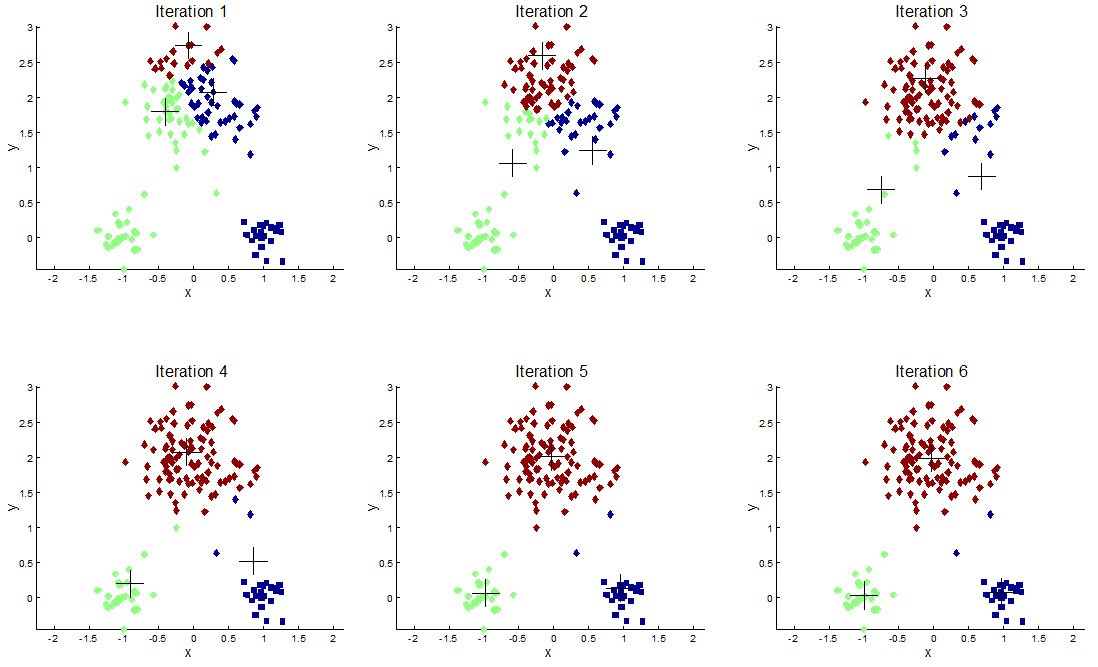
\includegraphics[width=0.80\textwidth]{kmeansclustering.jpg}
	\caption{Application de K-means}
	\label{fig:kmeansclustering}
\end{figure}

\newpage 
\tikz[remember picture,overlay]%
\node[fill=Sienna,text=white,font=\LARGE\bfseries,text=Cornsilk,%
minimum width=\paperwidth,minimum height=5em,anchor=middle]%
at (current page.middle){
\fbox{
\begin{minipage}{1\textwidth}
\textsl{\textsl{CHIFFRE CLÉ} \\
«\underline{15 minutes:} c’est le temps que met désormais Suravenir Assurances, du Crédit Mutuel, pour simuler les sommes à provisionner sur trente ans pour ses quelques deux millions d’emprunteurs, grâce aux technologies Hadoop. Hier, il fallait \underline{24 heures pour ce même calcul.}
»}  \\

\end{minipage}
} };
\end{center}

\newpage

\chapter*{Bibliographie \& webographie}
\begin{enumerate}
\item $http://blogs.msdn.com/b/big_data_france/archive/2014/06/17/un-peu-de-th-233-orie-pour-l-apprentissage-supervis-233-1-232-re-partie.aspx$
\item $http://blogs.msdn.com/b/big_data_france/archive/2014/06/17/un-peu-de-th-233-orie-pour-l-apprentissage-supervis-233-2nde-partie.aspx$
\item $http://blogs.msdn.com/b/big_data_france/archive/2014/06/06/un-peu-de-th-233-orie-pour-l-apprentissage-non-supervis-233.aspx$
\item $http://mathsmonde.math.cnrs.fr/images/pdf/part2/1-BigDataSmai.pdf$
\item $http://www.math.univ-toulouse.fr/~besse/Wikistat/pdf/st-m-app-intro.pdf$
\item $http://www.ey.com/Publication/vwLUAssets/EY-etude-big-data-2014/\$FILE/EY-etude-big-data-2014.pdf$
\item $http://www.strategie.gouv.fr/sites/strategie.gouv.fr/files/archives/2013-11-09-Bigdata-NA008.pdf$
\item $http://www.planet-data.eu/sites/default/files/presentations/Big_Data_Tutorial_part4.pdf$
\item $http://www.bigdataparis.com/guide/Guide_du_Big_Data_2013_2014.pdf$
\item $http://cr.g9plus.org/2014-12-16-G9plus-LB-Big-Data.pdf$
\item $http://www.decideo.fr/bruley/docs/Premiers\%20Pas\%20dans\%20les\%20Big\%20Data.pdf$

\end{enumerate}		
\chapter*{Conclusion}
Une explosion nécessite un contrôle et des outils sophistiqué pour la limiter et la gérer, c’est le même cas pour notre sujet « Big Data », on est devant une explosion d’information énorme, faut la gérer et la contrôler pour en tirer des informations qui vont nous servir dans beaucoup de domaines (prédiction, tracer et cibler,..). \paragraph{}
Comme nous l’avons vu dans le projet, le « Big Data » demande des algorithmes « big »  et puissant pour en profiter. Certes, ces algorithme ont des avantages et des inconvénient : demande plus de temps de calcul, sur-apprentissage,…Donc y a pas d’algorithme, pour l’instant, assez performant pour le « Big Data ». \paragraph{}
Grâce à la loi de Moore, expliqué dans le sujet, on pourrait avoir une idée sur l’avenir comment va être les machines et serveurs. La performance des machine augmente de plus en plus, ce qui garantirai qu’un certain temps, une machine qui pourra supporter le temps  de calcul. \paragraph{}
En effet, les ordinateurs quantique(processeur quantique à base de transistor quantique) est un espoir pour les informaticiens qui vont leur garantir leur besoins en terme de calcul et de performance. Comment ça se passe ?? \paragraph{}
Imaginons que vous cherchez un mot dans 10 livres. Les machines actuelles vont parcourir la recherche livre par livre, ça demande quelques milliseconde, mais imaginons avec un ordinateur quantique, la recherche est faite instantanément sur tous les livres à la fois, c’est extrêmement puissant, d’ailleurs ça va être le futur,  espérant. \paragraph{}
\\

\tikz[remember picture,overlay]%
\node[fill=Sienna,font=\LARGE\bfseries,text=Cornsilk,%
minimum width=\paperwidth,minimum height=10em,anchor=south]%
 at (current page.south) {Merci pour votre attention !};




\end{document}


\cleartoverso



%%%%%%%%%%%%%%%%%%%%%%
%% Back cover
%%%%%%%%%%%%%%%%%%%%%%

%% Temporarily enlarge this page to push
%% down the bottom margin
\enlargethispage{3\baselineskip}
\thispagestyle{empty}
%\pagecolor[HTML]{0C0303}
\pagecolor[HTML]{0E0407}

\begin{center}
\begin{minipage}{.8\textwidth}
\color{Cornsilk}\Large\bfseries
\lipsum[1]

%\begin{center}
%\huge\bfseries\sffamily\color{lime}`So Calming.'
%\end{center}

%\lipsum[2]

%\end{minipage}
%\end{center}

\vspace*{\stretch{1}}

\begin{center}
\colorbox{white}{\EANisbn[SC4]}

\vspace*{\baselineskip}

%\textbf{\textcolor{LightGoldenrod!50!Gold}{Malaysian \LaTeX\ User Group \textbullet\ \texttt{http://latex-my.blogspot.com}}}

\vspace*{\baselineskip}

%\textbf{\textcolor{LightGoldenrod}{Cover Illustration by Dusan Bicanski \textbullet\ \texttt{http://www.public-domain-image.com}}}
\end{center}
































\end{document}